\section*{Homework 5}

Do exercise 1-3 from AMPL book

\subsection*{A}

\noindent\textbf{Solution:}

Running the following code, \texttt{ampl.eval("Display Time, Make.rc")}, gives us the output below:

\begin{align*}
	\text{time}_{dv} &= 4640 \\
	\text{bands}_{rc} &= 1.80 \\
	\text{coils}_{rc} &= -3.14 \\
	\text{plates}_{rc} &\approx 0
\end{align*}

The interpretation of these values is as follows. First, time. If we were to add an extra unit of time (an hour) to availability we would see additional profit. To be precise we would see an increase of 4640 units of profit (dollar) per additional hour of availability. For bands, we see the same kind of thing. Every unit (ton) increase in the upper bound of bands made would see an increase of 1.80 dollars of profit. Coils has a negative coefficient. What this means is that every ton decrease in the lower bound of coils made would see an increase in profit by 3.14 dollars. This makes sense, we're maxing out the number of bands we can make and only producing the absolute minimum number of coils. Plates have a coefficient of 0, meaning that increasing or decreasing the bounds on its production would have no impact on profit. This also makes sense intuitively as production of plates falls within the provided bounds already. It is important to note that for these dual values and reduced costs, this relationship may not hold forever. These values are subject to change as constraints are modified.

\subsection*{B}

\noindent\textbf{Solution:}

The figures mentioned in the problem statement refer to the steel4 data and model files. Those have been shown earlier in the homework so I will not be showing them again. 

\begin{table}[h!]
\centering
\begin{tabular}{lcc}
\hline
 & \textbf{Steel3} & \textbf{Steel4} \\
\hline
Bands  & $6000$       & $\approx 3357.14$ \\
Coils  & $500$        & $500$ \\
Plates & $\approx 1028.57$ & $\approx 3142.86$ \\
Total Profit & $\approx 194828.57$ & $\approx 190071.43$ \\
\hline
\end{tabular}
\caption{Comparison of solution values and total profit for Steel3 and Steel4 models.}
\end{table}

To explain what's going on here we need to understand the new rate constraint. \texttt{reheat} has the same rate across all 3 products. What this means is that plates, with their very high profit coefficient of 2.9, outclass bands for this stage. Bands still come out on top for the rolling stage, which is why we still make so many bands, but this change is why we produce so much less of them.

\subsection*{C}

\noindent\textbf{Solution}

Using \texttt{amplpy} and saving the profit and reheat hours from each run gives us the following table:

\begin{table}[!ht]
    \centering
    \begin{tabular}{lcc}
    \hline
        reheat\_hours & profit & time\_dual\_value \\ \hline
        35 & 190071.43 & 1800.0 \\
        36 & 191871.43 & 1800.0 \\
        37 & 193671.43 & 1800.0 \\
        38 & 194828.57 & 0.0 \\
        39 & 194828.57 & 0.0 \\
        40 & 194828.57 & 0.0 \\
    \hline
    \end{tabular}
\end{table}


This table verifies what the problem statement wanted us to check. We have a constant dual value for reheating up until we hit 38 reheat hours. From there, it has no influence on our profit whatsoever. 

Next we check some other arbitrary values. We start with the provided $37 \frac{9}{14}$. To test this we also solve for $36 \frac{9}{14}$ so we can get the profit difference per unit difference. We also test just beyond this value and do the exact same process for $37 \frac{10}{14}$. 

This gives us the following results:

\begin{table}[!ht]
    \centering
    \begin{tabular}{lcc}
    \hline
        reheat\_hours & profit & time\_dual\_value \\ \hline
	$36 \frac{9}{14}$ & 193028.57 & 1800 \\\\ 
	$37 \frac{9}{14}$ & 194828.57 & 0 \\\\
    $36 \frac{10}{14}$ & 193157.14 & 1800 \\\\
	$37 \frac{10}{14}$ & 194828.57 & 0 \\
    \end{tabular}
\end{table}

These tables verify the problem statement. Results below that $37 \frac{9}{14}$ still show that 1800 profit increase. Right as soon as we surpass it even by a tiny amount we see diminishing returns.

One interesting observation is that $37 \frac{10}{14}$ doesn't actually see an 1800 profit increase despite the dual value of $36 \frac{10}{14}$. I wonder why that is. It must be that the slope at that point is still 1800, but the tiny part of $37 \frac{10}{14}$ that exceeds our threshold means we don't quite capture 1800 in profit for a one unit increase. This means the dual value doesn't quite tell the whole picture. 

\begin{figure}[htbp]
    \centering
    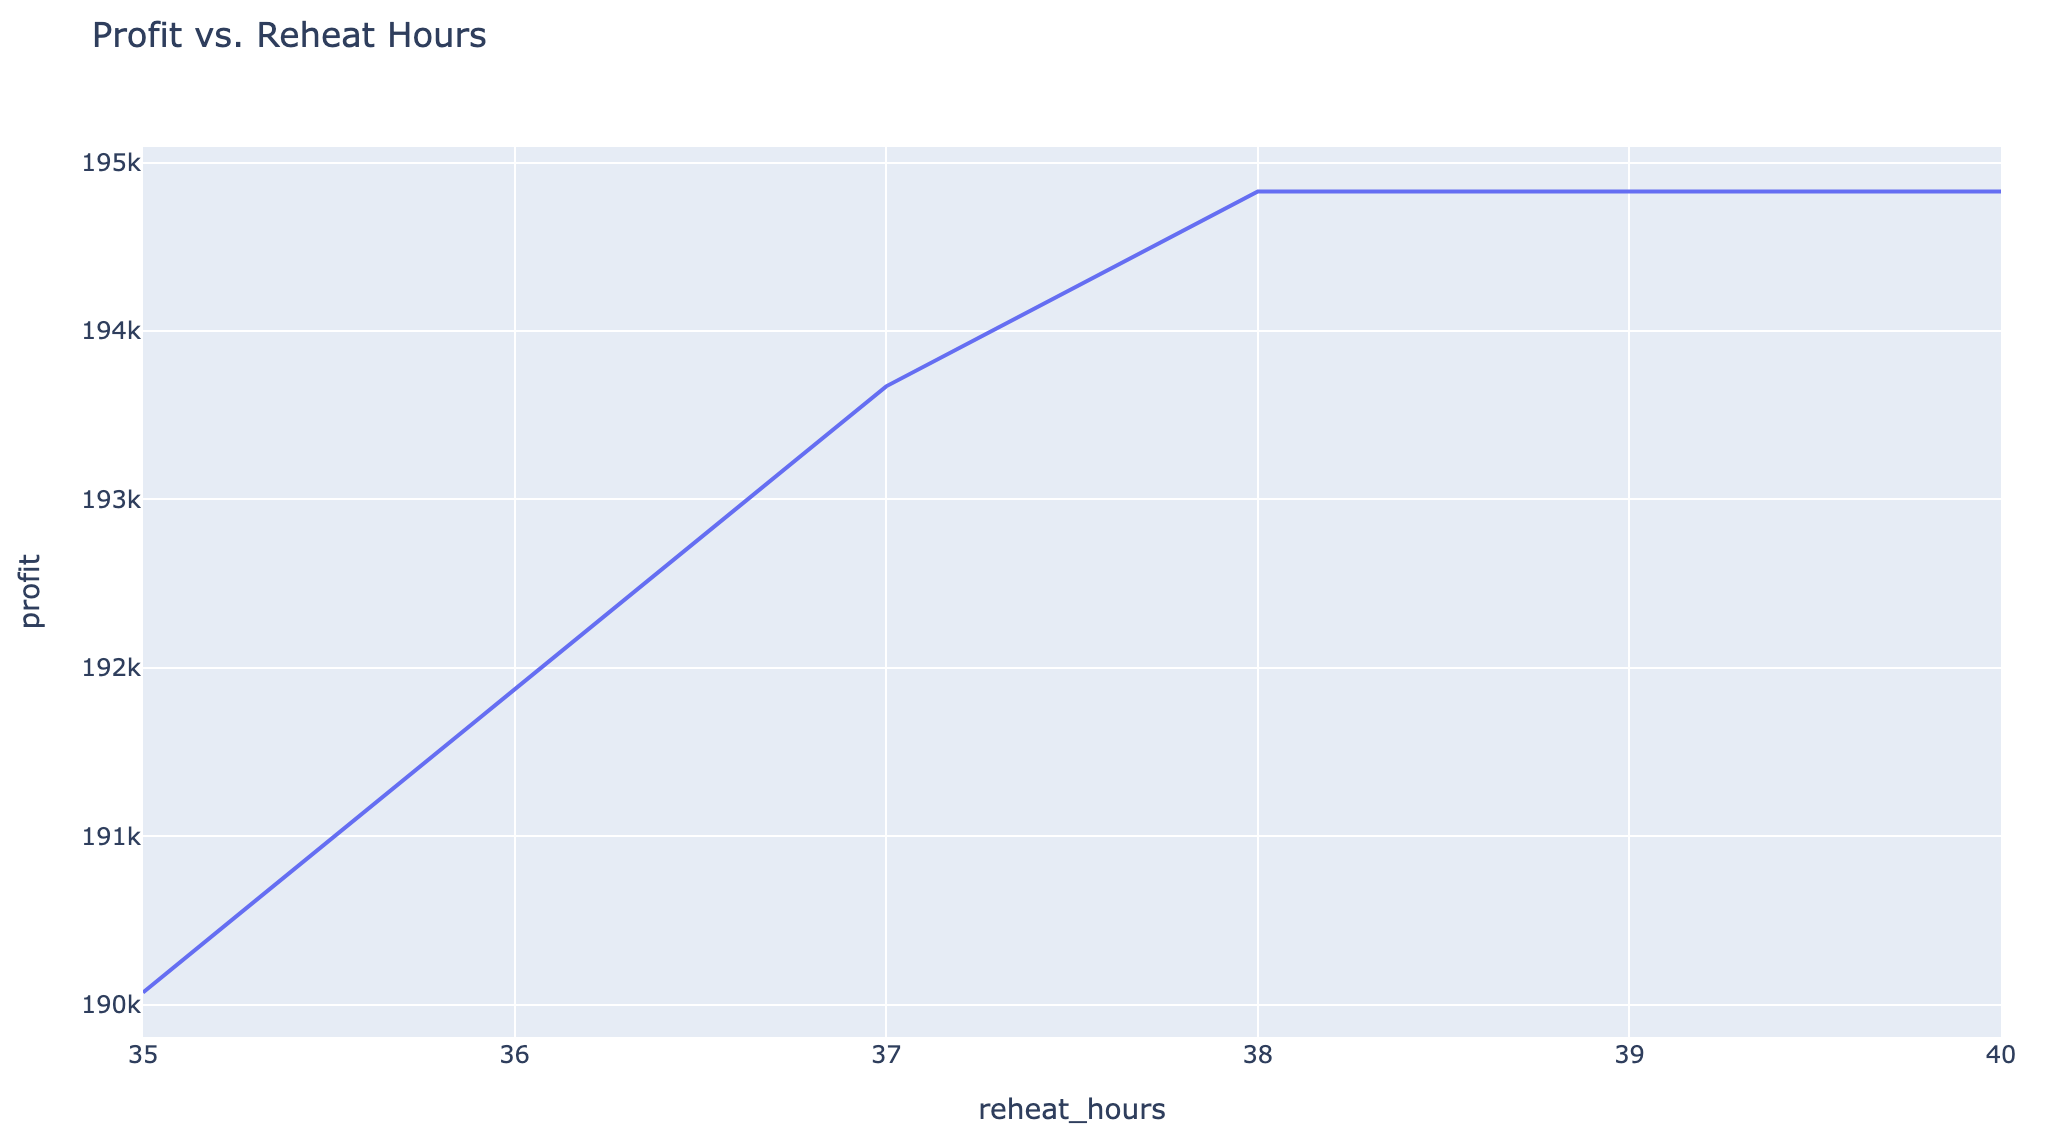
\includegraphics[width=0.8\textwidth]{../images/profit-vs-reheat-1.png}
    \caption{Plot created using the integer range of 35 through 40.}
    \label{fig:your_label}
\end{figure}

\pagebreak

\subsection*{D}

We extend the plot down to 25 reheating hours here.

\begin{figure}[htbp]
    \centering
    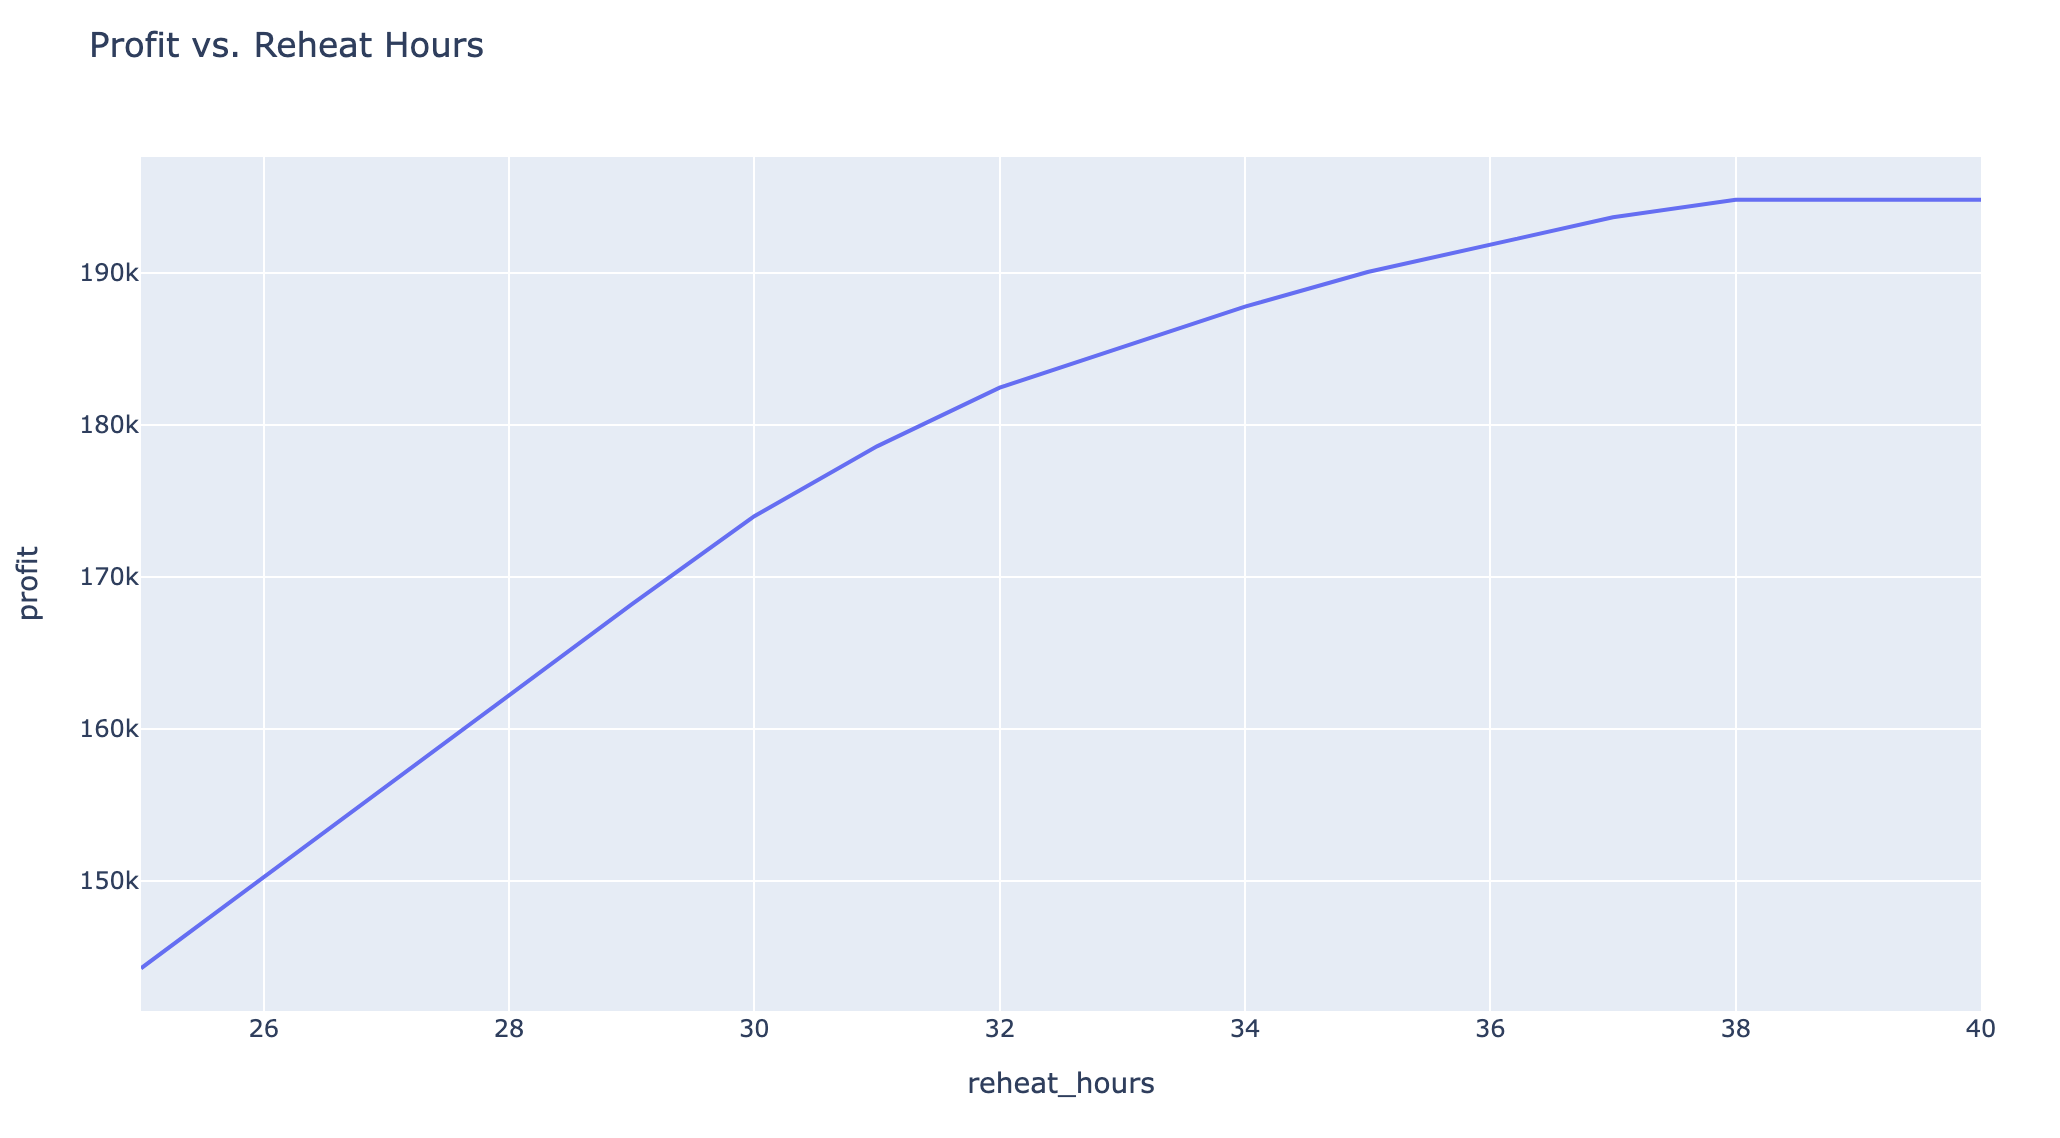
\includegraphics[width=0.8\textwidth]{../images/profit-vs-reheat-2.png}
    \caption{Plot created using the integer range of 25 through 40.}
\end{figure}

We also extend our table to show all of the profit changes as we move from 10 to 25 available reheating hours.

\begin{table}[!ht]
    \centering
    \begin{tabular}{lcc}
    \hline
        reheat\_hours & profit & time\_dual\_value \\ \hline
        10 & 0.0 & 0.0 \\
        11 & 0.0 & 0.0 \\
        12 & 66250.0 & 6000.0 \\
        13 & 72250.0 & 6000.0 \\
        14 & 78250.0 & 6000.0 \\
        15 & 84250.0 & 6000.0 \\
        16 & 90250.0 & 6000.0 \\
        17 & 96250.0 & 6000.0 \\
        18 & 102250.0 & 6000.0 \\
        19 & 108250.0 & 6000.0 \\
        20 & 114250.0 & 6000.0 \\
        21 & 120250.0 & 6000.0 \\
        22 & 126250.0 & 6000.0 \\
        23 & 132250.0 & 6000.0 \\
        24 & 138250.0 & 6000.0 \\
        25 & 144250.0 & 6000.0 \\
    \hline
    \end{tabular}
\end{table}


Here we have verified that from 12 available reheat hours to 25 hours we see a constant slope of 6000 dollars of profit per hour increase in availability. We also see 0s for 10 and 11 hours of availability. Why is that?

It's because of our minimum production constraints. In the steel4 data file, we have a commit parameter that controls our production lower bounds. We need a minimum of 1000 tons of bands, 500 tons of coils and 750 tons of plates.

Our time constraint is as follows:

\begin{lstlisting}
subject to Time {s in STAGE}:
   sum {p in PROD} (1/rate[p,s]) * Make[p] <= avail[s];
\end{lstlisting}

Running through the math for all products in the reheating stage:

\[
	\frac{1}{200} \cdot (1000 + 500 + 750) = 11.25 > 11
\]

Our minimum production requirements require more than 11 hours of reheating time, so anything below $11.25$ results in no feasible solution being possible. 
